\documentclass[letterpaper, 10 pt, conference]{ieeeconf} % Comment this line out
% if you need a4paper \documentclass[a4paper, 10pt,
% conference]{ieeeconf} % Use this line for a4
% paper

\IEEEoverridecommandlockouts{}
% This command is only needed if you want to use the \thanks command
\overrideIEEEmargins{} \let\labelindent\relax

% See the \addtolength command later in the file to balance the column lengths
% on the last page of the document



% The following packages can be found on http:\\www.ctan.org
\usepackage{graphics} % for pdf, bitmapped graphics files
% \usepackage{epsfig} % for postscript graphics files
% \usepackage{mathptmx} % assumes new font selection scheme installed
% \usepackage{times} % assumes new font selection scheme installed
% \usepackage{amsmath} % assumes amsmath package installed
% \usepackage{amssymb} % assumes amsmath package installed
\let\proof\relax \let\endproof\relax \usepackage{amsthm}
\theoremstyle{definition} \newtheorem{definition}{Definition}
\graphicspath{{images/}} \usepackage{xcolor,soul} \usepackage[inline,
shortlabels]{enumitem} \usepackage{biblatex} \renewcommand*{\bibfont}{\small}
% personal productivity
\usepackage[colorinlistoftodos]{todonotes} \presetkeys{todonotes}{inline}{}
\usepackage{hyperref} \newcommand{\toread}[1]{\todo[color=red!40!white]{#1}}
\newcommand{\towrite}[1]{\todo[color=blue!40!white]{#1}}
\renewcommand{\hl}[1]{{\color{red}#1}} \AtEveryBibitem{%
  \ifentrytype{book}{ \clearfield{url}%
    \clearfield{doi}%
    \clearfield{issn}%
    \clearfield{urldate}%
    \clearfield{review}%
    \clearfield{series}%%
  }{} \ifentrytype{collection}{ \clearfield{url}%
    \clearfield{doi}%
    \clearfield{issn}%
    \clearfield{urldate}%
    \clearfield{review}%
    \clearfield{series}%%
  }{} \ifentrytype{incollection}{ \clearfield{url}%
    \clearfield{doi}%
    \clearfield{issn}%
    \clearfield{urldate}%
    \clearfield{review}%
    \clearfield{series}%%
  }{} \ifentrytype{article}{ \clearfield{url}%
    \clearfield{doi}%
    \clearfield{issn}%
    \clearfield{urldate}%
    \clearfield{review}%
    \clearfield{series}%%
  }{} \ifentrytype{inproceedings}{ \clearfield{url}%
    \clearfield{doi}%
    \clearfield{issn}%
    \clearfield{urldate}%
    \clearfield{review}%
    \clearfield{series}%%
  }{} \ifentrytype{techreport}{ \clearfield{url}%
    \clearfield{doi}%
    \clearfield{issn}%
    \clearfield{urldate}%
    \clearfield{review}%
    \clearfield{series}%%
  }{} \ifentrytype{misc}{ \clearfield{url}%
    \clearfield{doi}%
    \clearfield{issn}%
    \clearfield{urldate}%
    \clearfield{review}%
    \clearfield{series}%%
  }{} }

\bibliography{rexam.bib}

\title{\LARGE \bf A Taxonomy for Characterizing Modes of Interactions in
  Goal-driven, Human-robot Teams }
\newcommand{\citet}[1]{\citeauthor{#1}~\cite{#1}}
% \author{ \parbox{3 in}{\centering Huibert Kwakernaak*
% \thanks{*Use the $\backslash$thanks command to put information here}\\
% Faculty of Electrical Engineering, Mathematics and Computer Science\\
% University of Twente\\
% 7500 AE Enschede, The Netherlands\\
% {\tt\small h.kwakernaak@autsubmit.com}} \hspace*{ 0.5 in} \parbox{3 in}{
% \centering Pradeep Misra**
% \thanks{**The footnote marks may be inserted manually}\\
% Department of Electrical Engineering \\
% Wright State University\\
% Dayton, OH 45435, USA\\
% {\tt\small pmisra@cs.wright.edu}} }

\author{ Priyam Parashar, Lindsay M. Sanneman, Julie A. Shah, Henrik I.
  Christensen }


\begin{document}



\maketitle
\thispagestyle{empty} \pagestyle{empty}


%%%%%%%%%%%%%%%%%%%%%%%%%%%%%%%%%%%%%%%%%%%%%%%%%%%%%%%%%%%%%%%%%%%%%%%%%%%%%%%%
\begin{abstract}
  This document contains the edits to the taxonomy as well as the changes to a
  priori sa framework. Additionally, the a priori sa is then further intertwined
  into the dynamic factors of the taxonomy to create a more grounded framework.
\end{abstract}


%%%%%%%%%%%%%%%%%%%%%%%%%%%%%%%%%%%%%%%%%%%%%%%%%%%%%%%%%%%%%%%%%%%%%%%%%%%%%%%%

\section{Edits to Taxonomy}

\subsection{Additions}

The main article that I found and had material contributions to the taxonomy is
the one by \citet{moya2007towards}. The taxonomy takes a holistic view of a
multi-system environment and considers the following three components as overall
description of the system:
\begin{itemize}{}
  \item Situated environment
        \begin{itemize}{}
          \item Closure --- If agents defined outside the system can still affect
                the R environment
          \item Dynamism --- Whether the environment is affected by just the system
                (static) or because of randomness/open environment (dynamic)
          \item Determinism --- If actions always have a deterministic outcome over
                time, sort of like environment stationarity
          \item Cardinality --- Size of environment, affected agents and objects
                (finite, finite uncountable, infinite, etc.)
        \end{itemize}
  \item Population
        \begin{itemize}{}
          \item Size
          \item Diversity
          \item Homogeneity
          \item Goal structure
          \item Cooperability
        \end{itemize}
  \item Agent characteristics
        \begin{itemize}{}
          \item Reasoning
          \item Perception
          \item Action
        \end{itemize}
\end{itemize}

I found multiple evidence in the literature that capabilities are always
abstracted one way or the other. We can leverage this trend to propose mobile,
perception and reasoning bins which if present/absent represent an agent's
capabilities. TK:\@ references of papers I found this in. The paper mentioned in
the previous paragraph also has a taxonomy spelling out bins for perception and
communication categories.

To bring back the papers we have already included, I thought the
\texttt{phys\_proximity} categories in \citet{Yanco2004updated} made a lot of
sense for associating the environment or workspace configurations to the
physical nature of tasks.

\subsection{Changes}
\begin{itemize}{}
  \item ``Criticality'' should be further broken down into risk versus mission
        criticality. Mission criticality can be grounded into Lindsay's co-design
        method while the risk scale can be better informed by robot risk scales.
  \item Another thing I realized was that environment is too broad a category,
        maybe that is why we never saw much specification for it. Might we change
        ours to ``situated workspace''. I think this terminology has better relation
        to what we actually define in our taxonomy.
  \item Given that levels of autonomy divides levels between sensing, acting and
        planning, we should maybe expand the Cognitive Task Nature category further
        into perception and reasoning.
  \item We should also use a running example (maybe one of the two from the
        case-study section) to ground our abstract statements into something
        intuitive. Maybe we can use the complex capture-the-flag example as the main
        running example while the rest is just added to provide different viewpoints
        from different domain perspectives.
\end{itemize}

\section{A Priori Situational Awareness Framework for Stereotyping Human Roles}

This section introduces a bridging framework, grounded within the taxonomic
factors defined in the previous section, which helps in assessing if the system
design fulfills the mode of interaction that is established between the human
and the robot. We do this by stereotyping the expected knowledge levels of the
human collaborator, stereotyped in a certain role within the boundaries of the
specified system, and compare this with the required knowledge associated with
the successful execution of the interaction relationship. We categorize these
knowledge levels along the same main axes which we used to establish our
taxonomy, i.e., task-work knowledge, team-work knowledge, and
environment/situated-workspace knowledge. As we mentioned earlier, the axes
defined are not entirely independent of each other, there is some effect either
of scope or of correlation which exists between the task being done and the
workspace or the team choices for it, or vice versa. This section helps in
understanding these relationships and organizes them in a tier-based framework
of knowledge levels.

Depending upon the \texttt{focus} of the task and whether the task is operating
in normal or subnominal state, one can establish the \texttt{nature} of
interaction that will be required to complete the task-work. Let's consider the
capture-the-flag example the area coverage sub-task is one which requires mainly
physical cooperation within the team. On the other hand, a defend-the-flag
sub-task, which is of physical nature when a strategy is already agreed upon,
can switch to a sub-nominal state when the defense perimeter is breached and is
elevated to a cognitive task where a new strategy needs to be decided on before
being physically actuated by the players. A change in the nature of team-work
inevitably entails a subsequent change in the nature of communication between
the players, which means a different set of sensing and reasoning capabilities
are required for the changed sub-task. The design of an HRI system should be
able to satisfy the largest such set of mobile, perception, and communication
capabilities as well as the infrastructure to establish the required information
exchange protocols. In a very similar way, depending upon the team-work between
a human and a robot depending upon if the interaction is established with a peer
or a supervisor and whether it is in nominal or sub-nominal status, a similar
set of rules dictate a necessitated change in the quality of information being
exchanged between the two interactants. This section stereotypes the roles
defined in \citet{Goodrich2007,Scholtz2003} by grounding their expected
knowledge levels for interactions to hold up in nominal conditions. This also
creates a hard boundary of what can be considered a sub-nominal state of
interaction and might require a change in the edges of the interaction graph
where interactants are nodes and an edge exists between two nodes if they are
interacting.

We call this an a priori situational awareness framework because it is heavily
inspired by the situational awareness framework by \citet{Endsley1995}, but
considers the a priori assumptions which are placed on a system before its
deployment and their effects on the situational awareness of a dynamic system
during execution. The a priori situational awareness framework also acts as a
switchboard connecting task, team and workspace specification to the allowable
ranges of levels of autonomy for the robot as well as the level of information
abstraction or the quality of information that should be exchange between the
interactants. This is done by taking a sub-task, describing it based on the
taxonomic factors already provided, creating a set of categorical knowledg
levels that we can expect the human interactant to possess, and then finally
relating these categories with the expected level of autonomy for that
interaction as well as the information abstractions which should be considered
for maximum efficiency of knowledge take-up. We first begin by introducing the
knowledge levels which will be used to stereotype the human interactant in a
system.

\towrite{Need to bring out the relation of a priori sa with sa framework and
  Donald Norman's interaction model}

\subsection{Knowledge Levels for Stereotyping Human Roles}

We will typify each role by assigning their:
\begin{itemize}
  \item Expected task-work knowledge level which corresponds to the task nature
        taxonomy,
  \item Expected team-work knowledge which relates to their mental model of the
        robot's mechanisms (similar to Donald Norman's mental model axis of the
        interaction model)
  \item Expected workspace knowledge which helps assess if the current
        interactant has the right abstractions and knowledge in case of
        environmental changes during operation
\end{itemize}

\subsubsection{Task-work Knowledge of Human Interactants}
This knowledge level corresponds to the \textit{Signifiers} aspect of Norman's
interaction model. Signifiers in his model define what kind of relationships can
be established between the object and the agent. In our framework similarly the
task knowledge is a ``signifier'' describing if the current sub-task can be
collaborated on with the selected human.

\towrite{in the following list also add 1 example per bin of the scale}

This is a uni-dimensional scale which is organized into the following bins:
\begin{itemize}{}
  \item \textit{ Physical or tactical } knowledge about actuating the sub-task
        which is necessary for a task of physical nature
  \item \textit{ Conceptual or operational } knowledge about which features in
        the environment, and the team collaboration affect the subtask. We map this
        level to cognitive-perceptual nature of tasks as such roles have an
        understanding of which features from the environment or team must be
        included or excluded for the task to be successful, thus affecting the
        short-term execution and interactions.
  \item \textit{ Strategic } knowledge about the over-arching mission
        priorities, which is mapped to cognitive-reasoning nature of tasks.
  \item \textit{ Social } knowledge about the outward appearance of the system,
        which is mapped to social nature of sub-tasks.
\end{itemize}

\subsubsection{Team-work Knowledge of Human Interactants}
This knowledge level corresponds to the \textit{Conceptual Model} aspect of
Norman's interaction model. The agent should have a, not complete but, good
enough mental model of the mechanisms of the object such that the intended
interaction can be successfully executed. In our framework this relates to the
expected mental model that a human, in a given role, should have of the robot
such that the intended interaction, as stereotyped by the role, can be
successfully established and executed. In the following bins everytime we mean
the knowledge of something with respect to the robot's mechanisms. Going from
most sparse to most dense mental model:
\begin{itemize}{}
  \item \textit{None} --- The only knowledge is conditioned on the form or
        appearance of the robot, thus making roles with this kind of knowledge more
        suitable for sub-tasks which do not require specialized knowledge.
  \item \textit{Functional} --- Knowledge of the physical and reasoning
        capabilities and limitations, which makes roles at this level more
        appropriate for goal-setting and resource management tasks in the system.
  \item \textit{Behavioral} --- Knowledge of how the physical behaviors and
        reasoning capabilities manifest together to fulfill functionality. The roles
        at this level have enough knowledge to participate and intervene with the
        planning and actuation system of the agent.
  \item \textit{Internal} --- Knowledge of how the physical and cognitive
        behaviors, interactions and commands affect the internal state and
        vice-versa. Usually the mental model assigned to developers and debuggers of
        the software and the hardware.
\end{itemize}

\subsubsection{Work-space Knowledge of Human Interactants}
This is a new scale, different from Norman's model, as robots operate in
situated environment therefore affecting and being affected by the environment.
This scale quantizes the expected expertise or knowledge that a human should
have of the environment and objects in the environment such that the intended
interactions can be established with a common understanding of the workspace. It
should be noted that all of these knowledge levels mention the expectation but
are not hard-rules for each kind of interaction. For example, in the USAR case
it would be great to have an operator who has full knowledge about the
underground debris and crash-site map, however this is not possible. Therefore
the most viable operator would be the one with past experience of such missions
and understanding of how the robot represents environments and its artifacts
(behavioral mental model). Going from most to least knowledge levels:
\begin{itemize}{}
  \item \textit{Exact Knowledge} --- The human has worked in the exact
        environment with the exact artifacts before
  \item \textit{Heuristic Knowledge} --- The human has worked in similar
        environments before and possesses heuristic knowledge of how to operate in
        it
  \item \textit{No Knowledge} --- The current environment is entirely new to the
        human

\end{itemize}

\subsection{Stereotyping Roles Grounded in APSA Knowledge Levels}

The three categories or axes described in the previous section provide the
guiding functions to the questions of whom to address a task, team or
environment-centric issue to, what level of guidance to expect in return and at
what level of abstraction should the current state of the robotics agent be
translated to so that it makes sense to both the interactants.
\citeauthor{Scholtz2003} in her \citeyear{Scholtz2003} paper does a similar
analysis of roles with respect to the 7 layer HCI model proposed by Donald
Norman, the current work is a natural extension of the same grounding it in
taxonomic bins and knowledge structures for dynamic evaluation.

We propose the following stereotypes of roles to answer these questions:
\begin{itemize}{}
  \item \textit{Operator} --- The operator is a software debugger who ensures
        that the robot is reacting to the behavioral and high-level commands as it
        should. This necessitates that internal knowledge of the mental model of the
        robot is necessary, exact (sandboxed experiments) to heuristic knowledge
        about environment, some physical and rigorous operational task knowledge
        necessary.
  \item \textit{Mechanic} --- Like an operator but debugs hardware with software
        interventions and hooks. Similar stereotype as operator, rigorous physical
        knowledge required.
  \item \textit{Peer} --- Peers usually interact with the agent to change or
        update its short-term goals and plans, or to help with the execution of
        short-term actions within the boundaries of the priorities set by the
        supervisor. In theory, the distinctions between peer, supervisor and
        teleoperators is very fuzzy however for the purposes of the current paper we
        make a firm distinction where peers strictly collaborate in a shared-control
        fashion, i.e.\ collaboration when the machine requires it independent of
        whether it was human-initiated or robot-initiated and the peer has no say in
        the overarching goals and purpose of the robot. This necessitates that
        functional to behavioral mental model required depending upon degree of
        collaboration, mostly uses visual or higher-level communication cues to
        interact, exact to heuristic knowledge of environment. Novel environment
        collaborations are possible where the peer has zero environmental knowledge,
        but not very common in current HRI landscape. Usually have operational
        knowledge of tasks being undertaken, treated as experts, or at least
        experienced, in most of current literature. Certain studies treat them as
        non-experts but the learning or collaboration in such context is strictly
        limited to only a physical nature.
  \item \textit{Supervisor} --- Can be further broken up into:
        \begin{itemize}{}
          \item \textit{Teleoperator} --- At this end of the supervisor spectrum the
                machine and the human have a physical coupling, which could manifest
                directly or via some teleoperated interface and device. The goal
                decisions are strictly within the reign of the operator while the
                sensing and actuation support is provided by the robot. Teleoperators
                need to have at least a behavioral knowledge of the robot's mechanisms
                specially when the machine affords limited autonomous corrections over
                teleoperators commands, to maintain transparency. Additionally, the
                teleoperator should be trained in the physical or tactical actuation of
                the task at hand and needs at least a heuristic knowledge of the
                environment to understand how to most efficiently steer the robot.
          \item \textit{Mission Supervisor} --- This is the more sophisticated end
                of the supervisor spectrum and is defined by the existence of strictly
                high-level communication between the human and the robot. Mission
                supervisor can not only switch to the teleoperator spectrum, provided
                they have the prerequisite know-how of the physical limitations of the
                robot, to actuate a task but can also change the overarching priorities
                of the machine to substantially change their plans and goals. Such a
                drastic shift in the machine's goals and plans should not be afforded to
                any other role. Under the provided definition the mission supervisor
                should have at least a functional knowledge of the robot's mechanism, at
                least a heuristic knowledge of the environment and is expected to hold a
                strategic knowledge of the current task for the given domain.
        \end{itemize}
  \item \textit{Mentor} --- This role was introduced to define a robot's
        behavior when it is deployed as the subject matter expert to monitor, train
        or educate human interactants. Depending upon the domain of interaction the
        mentorship can vary anywhere from a physical to cognitive to social nature.
        However, in any case the robot will be expected to have an exact knowledge
        of the environment and at least a functional level of knowledge about how
        the human interactants process the commands, corrections and instructions
        provided by the robot. This is where Theory of Mind models come into play
        when deciding on the level of sophistication of robot programming.
  \item \textit{Information Consumer} --- An information consumer may or may not
        have stake in the mission being executed by the robot, however it is
        expected that the human, or computing agent, will have a deep enough
        knowledge about the overall structure of the mission such that he/she/it can
        assimilate the data in an informative way. Therefore, it is expected the
        information consumer will at least have a conceptual knowledge about the
        tasks of the mission, possesses at least a functional knowledge of the
        robot's mechanism to make sense of the data being provided, and can be
        expected to operate in a novel environment.
  \item \textit{Bystander} --- A bystander is someone external to the defined
        mission domain and definitions.
\end{itemize}

\subsection{A Priori Situational Awareness and Taxonomic Effects}

Now that we have stereotyped each role, we can hierarchically categorize the 10
LoRAs into ranges which are applicable to perception versus physical versus
reasoning tasks. Depending upon the criticality of the task the agents can now
dynamically decide on which side of the LoRA spectrum should the robotic agent
operate.

Similarly, the mental model scale of APSA framework directly corresponds to
levels of information abstraction:. I suggest doing one mini review to find out
how plans or instructions are abstracted in robotics literature and connect the
mental models with those abstraction tiers. The overall process flow is
described in the following diagram:

\begin{figure}[t!]
  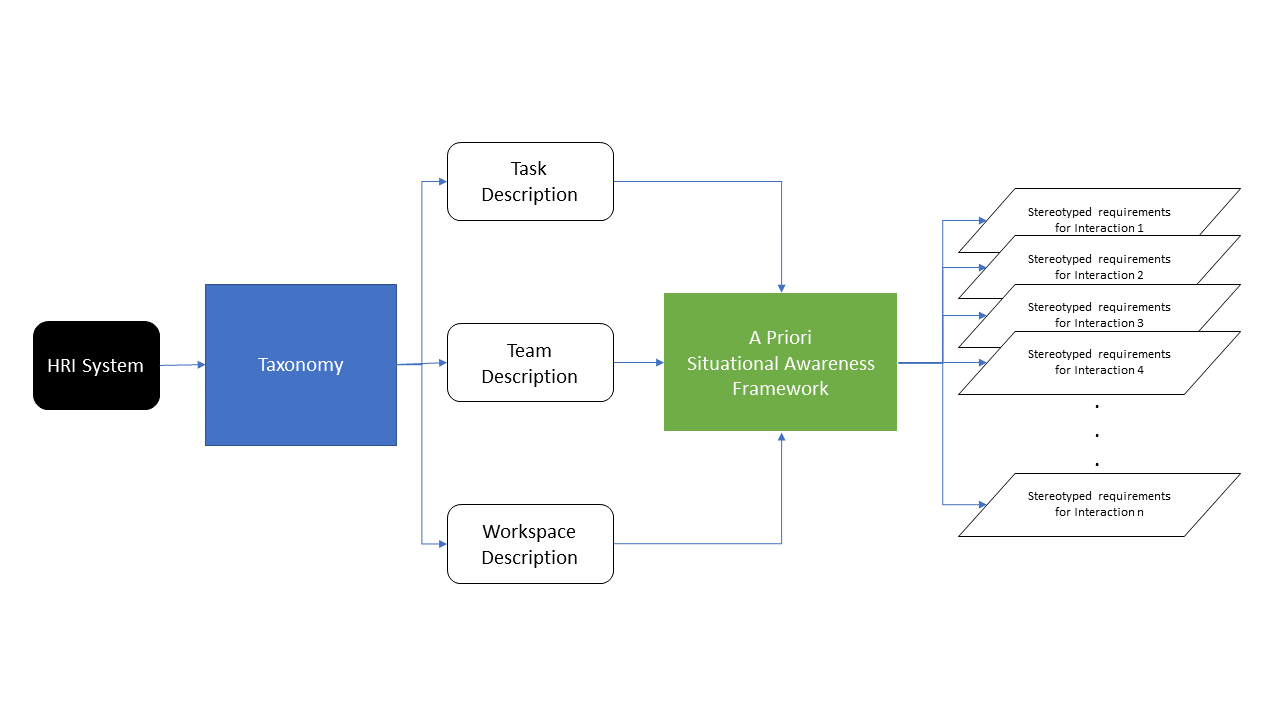
\includegraphics[width=0.9\textwidth]{apsa.png}
  \caption{Process Flow from Taxonomy to Interaction Requirements}
\end{figure}

\begin{table*}[b!]
  \caption{Julie's Comments}
  \begin{tabular}{p{8cm} p{8cm}}
    \toprule                                                                                               \\
    \textit{Comment}                                            & \textit{Response}                        \\
    \midrule                                                                                               \\
    A. Does this task axis related to ``Knowledge'' or he task? Do you mean tactical knowledge on how to
    perform a task? When I saw the category task I thought you would be defining characteristics of
    the task, rather than knowledge for different ways to do it & This makes me think we should
    have a better introduction to what does the A priori SA mean and does in the current scope             \\
    B. Multiple comments on clarity of role definition          & This draft will focus on this            \\
    C. Why is a certain knowledge level lowest or highest?      & There should be either a diagram or some
    reference to the taxonomy to make this more intuitive                                                  \\
    \bottomrule
  \end{tabular}
\end{table*}

\end{document}

% LocalWords: Signifiers
